\chapter{Análisis de generadores de datos\label{02estadoArte}}

\section{Características de herramientas de generación de datos}

En la actualidad podemos encontrar generadores de datos por la web que trabajan a través de una API para generar objetos con atributos predefinidos y grandes conjuntos de datos. Estos objetos además pueden ser exportados a una gran variedad de formatos de objetos como XML, JSON, CSV, TXT o directamente se pueden almacenar en algunas bases de datos muy populares como MySQL u Oracle DB.

Algunas de estas Webs son:

\begin{itemize}

	\item \textbf{\href{https://mockaroo.com}{Mockaroo}}: Esta herramienta tiene una interfaz de usuario sencilla e intuitiva, lo que la hace muy buena opción para aquellos usuarios que quieren un conjunto de datos rápido y personalizado sin tener que descargar ni profundizar conocimientos en el asunto.


	\begin{figure}[h!]
		\centerline{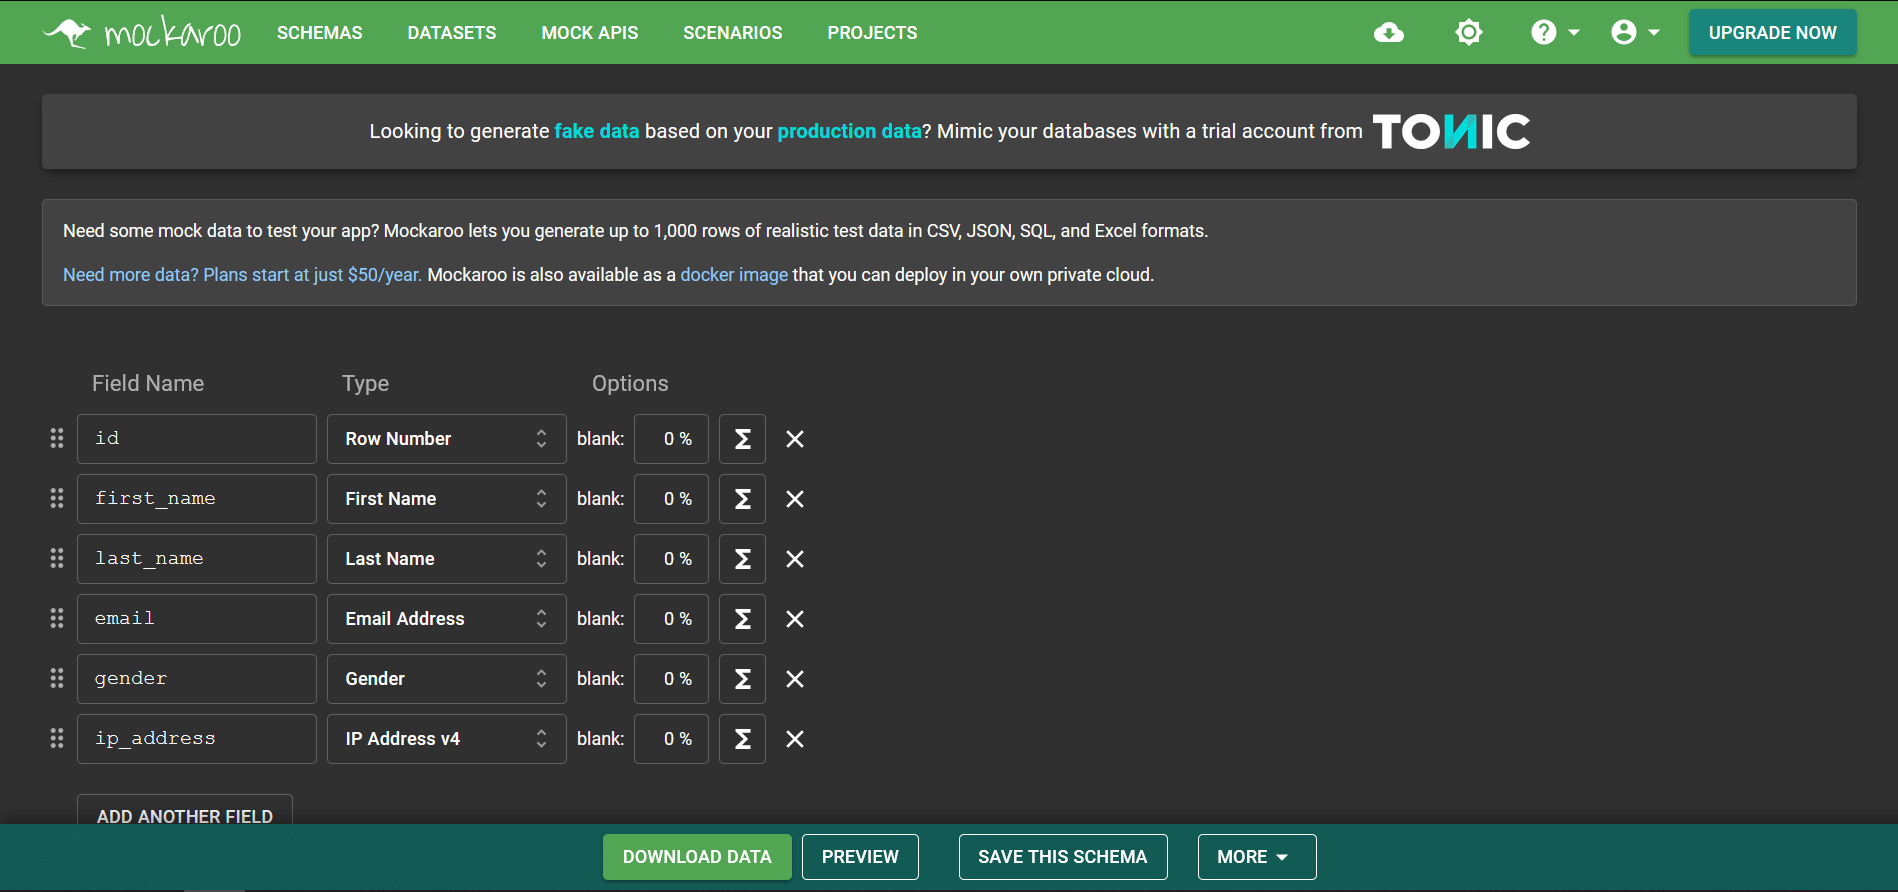
\includegraphics[width=1\textwidth]{mockaroo.png}}
		\caption{Ejemplo de configuración de generación de la herramienta Mockaroo.}
		\label{figure:mockarooWeb}
	\end{figure}

	En la figura~~\ref{figure:mockarooWeb} se muestra un ejemplo de configuración para la generación de entidades con 6 atributos de los que se puede definir nombre del campo, el tipo de dato, un porcentaje de nulo y alguna operación especial.

	En este generador podemos construir hasta 1000 filas de manera gratuita definiendo para cada columna su nombre, tipo, porcentaje de blanco o nulo y una última opción más avanzada que nos permitirá realizar algunas operaciones con los datos generados como funciones, sumatorios, etc. Además permite la exportación en los formatos CSV, JSON, SQL, Excel, XML, TXT y la inserción directa en Cassandra CQL.

	Como punto negativo además de la limitación de 1000 filas que, como veremos más adelante, puede ser crucial para el desarrollo de software, medidas de rendimientos, etc. Cabe destacar que, aunque la aplicación nos ofrece una gran variedad de conjuntos de datos, no nos permite la posibilidad de aportar uno propio; lo cual podría ser de gran ayuda a la hora de ofrecer datos más realistas como nombres o apellidos de ciertos territorios.


	\item \textbf{\href{https://generatedata.com}{GenerateData}}: A diferencia de Mockaroo, este es un proyecto de código abierto mucho más amplio. Destaca su web, la cual es accesible de primera mano, y aunque la experiencia de usuario es algo más negativa que \textit{Mockaroo} podemos obtener alguna ventaja.

	\begin{figure}[h!]
		\centerline{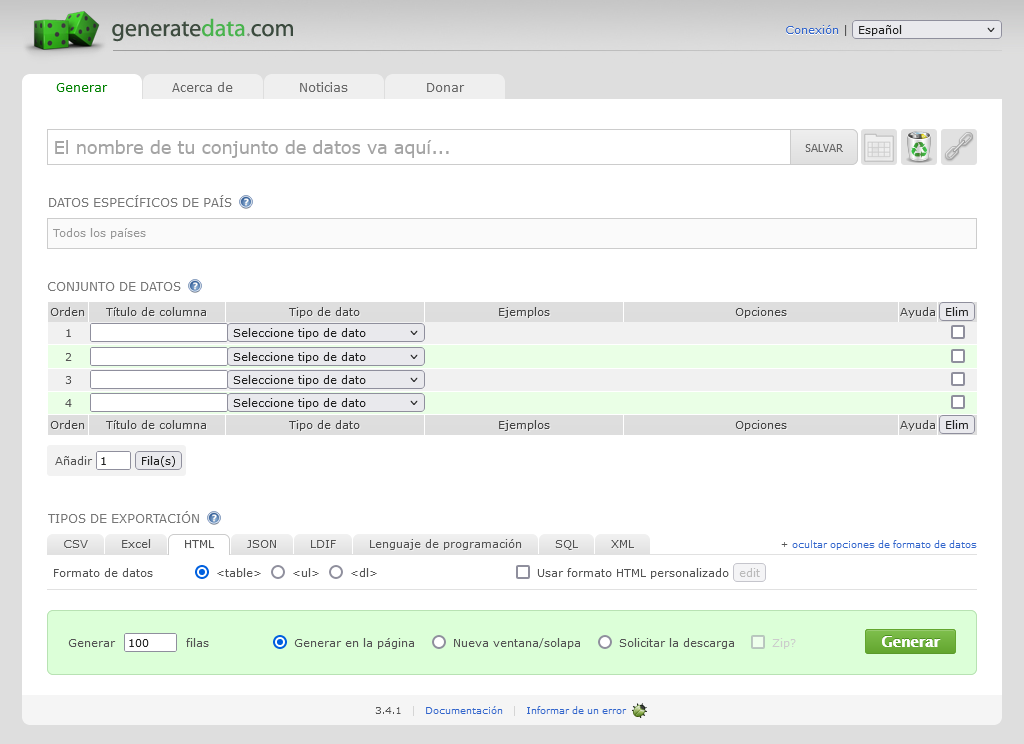
\includegraphics[width=1\textwidth]{generateData.png}}
		\caption{Ejemplo de configuración de generación de la herramienta Generate Data.}
		\label{figure:generateDataWeb}
	\end{figure}	

	Las opciones de la herramienta son muy parecidas en la figura~\ref{figure:generateDataWeb} se puede observar la definición de un esquema fijo con una generación de datos aleatorio a través de unos subconjuntos de datos, exportación en varios formatos: CSV, JSON, XML.

	Actualmente el número de filas no se puede modificar y queda a 100 por defecto, si queremos obtener más filas será necesario realizar una donación para poder obtener un usuario con estos privilegios. Sin embargo, este proyecto se puede descargar de forma local y de esta manera acceder a la cantidad de filas que el usuario requiera. Además podemos utilizar la \textbf{\href{http://benkeen.github.io/generatedata/api.html}{API}} de generateData para poder acceder a su generador de datos desde cualquier proyecto independiente.

	El proyecto es open source y se puede colaborar a través de su repositorio en \textbf{\href{https://github.com/benkeen/generatedata}{GitHub}}.

	\item \textbf{Otros generadores}: Existen varios generadores de datos que vamos a agrupar aquí debido a que comparten algunas características como estar embebidos en programas de gestión de bases de datos comerciales, ser de pago y no pertenecer a proyectos open-source. Algunos de estos son: \href{https://www.datprof.com/}{DatProf}, \href{https://www.red-gate.com/products/sql-development/sql-data-generator/}{Redgate SQL Data Generator}, \href{https://www.sqlmanager.net/products/mysql/datagenerator}{EMS Data Generator} y \href{https://www.datanamic.com/datagenerator/}{Datanamic Data Generator MultiDB}.

	\end{itemize}


\subsection{Limitaciones de las herramientas existentes}

Los generadores de datos actuales suelen partir de un conjunto de datos almacenados, escogiendo de forma aleatoria entre estos para crear nuevos conjuntos de datos. El problema es que la limitación de este conjunto de datos provoca que el resultado final sea muy sintético y se aleje de las diversas formas e infinitas posibilidades que una base de datos real puede adoptar.

La generación de datos actual deja a un lado las bases de datos NoSQL, lo cual es un problema para muchos proyectos tanto académicos como industriales que necesitan de estos nuevos sistemas de almacenamiento para desarrollar, testear y comparar sus bases de datos.

Los generadores de datos antes vistos siguen esquemas marcados de generación, lo cual es óptimo para bases de datos esquemáticas como las relacionales; sin embargo, son un problema para testear posibles errores en bases de datos NoSQL. Con la generación de datos schemaless se debe soportar la existencia de variaciones estructurales para una misma entidad: campos que no aparecen en todos los objetos o campos que pueden tener diferente tipo, además de propiedades vacías o nulas como se pueden ver también en bases de datos relacionales. 

Pongamos como ejemplo que queremos crear una entidad que represente a un trabajador de una gran empresa internacional que tiene como atributos el campo name, address y email, se ha diseñado una aplicación para la gestión de estos usuarios (creación, consulta y modificación) y para favorecer la evolución de la aplicación se ha pensado que la dirección de correo puede tomar distintos tipos de datos, una cadena con la dirección o un array de direcciones si el trabajador tiene varios correos, además el atributo de la dirección se ha definido como un string para las direcciones locales "calle-número-planta-puerta" pero también puede tomar forma de objeto si la dirección no es local e incluso ser una colección de direcciones si el trabajador tiene más de una propiedad y estas direcciones ser a su vez cadenas u objetos


\begin{figure}[h!]
	\centerline{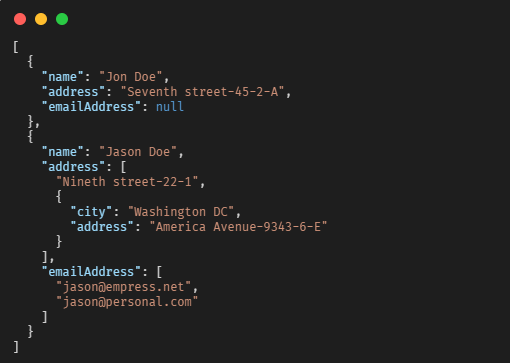
\includegraphics[width=1\textwidth]{exampleJson.png}}
	\caption{Ejemplo de generación de datos para entidades con variación de tipos.}
	\label{figure:jsonExample}
\end{figure}

La figura \ref{figure:jsonExample} sería un ejemplo de una generación de dos entidades. El problema reside cuando la empresa que ha creado la aplicación debe realizar tests para aplicar en una base de datos que crecerá de forma masiva. Podrá realizar pruebas sobre pequeñas porciones de datos pero no podrá depurar sobre una base de datos de la magnitud que en un futuro albergará.

También todas estas opciones dejan de lado la interrelación de las entidades lo cual es necesario puesto que una base de datos es un conjunto de datos que está relacionado desde entidades del mismo tipo hasta otras de tipos distintos. Vamos a modificar nuestro ejemplo anterior para añadir un identificador a nuestras identidades y un atributo jefe que sea una referencia a otra entidad trabajador.


\begin{figure}[h!]
	\centerline{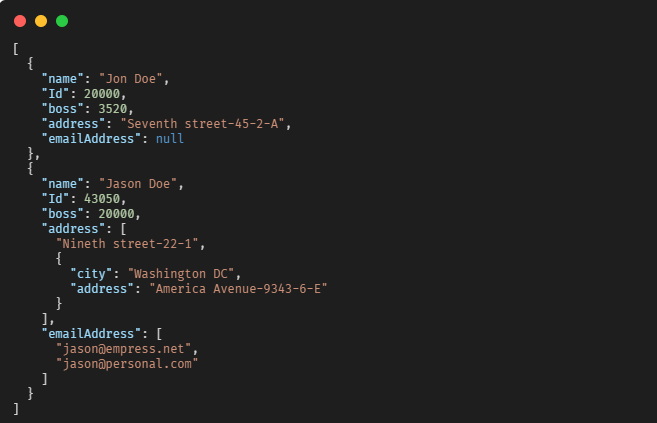
\includegraphics[width=1\textwidth]{exampleJson2.png}}
	\caption{Ejemplo de generación de datos para relaciones de entidades.}
	\label{figure:jsonExample2}
\end{figure}

En la figura~\ref{figure:jsonExample2} apreciamos que en este caso sería imposible para la empresa realizar una generación masiva de datos como la del ejemplo debido a que las herramientas existentes crean entidades independientes unas de otras.

Por último, destacar que los ejemplos vistos anteriormente carecen de pseudoaleatoriedad, por lo que no sería posible replicar una generación de entidades aleatorias vista anteriormente algo que puede ser de gran utilidad si un conjunto de datos ha sido modificado y se quiere recuperar su estado original o compararlo con el transformado.

%%% Local variables:
%%% TeX-master: "memoria.tex"
%%% coding: utf-8
%%% ispell-local-dictionary: "spanish"
%%% TeX-parse-self: t
%%% TeX-auto-save: t
%%% fill-column: 75
%%% End:

%  LocalWords:  Scala interoperabilidad metamodelado metamodelo Ecore
%  LocalWords:  Sirius
